\documentclass[10pt]{article}
\usepackage[margin=0.85in]{geometry}
\usepackage[T1]{fontenc}
\usepackage[utf8]{inputenc}
\usepackage{lmodern}
\usepackage{amsmath,graphicx,array,longtable}
\usepackage[hidelinks]{hyperref}
\setlength{\parindent}{0pt}
\setlength{\parskip}{5pt}
\setlength{\emergencystretch}{3em}
\title{When Tool Calls Succeed but Manipulation Does Not: An Evidence Audit of Guava on Piper}
\author{Guava-on-Piper working technical report\\Human author metadata to be finalized}
\date{23 October 2026}
\begin{document}
\maketitle

\textbf{Working draft, 23 October 2026. Authors and affiliations to be finalized by the repository owner. Not submitted, peer reviewed, or accepted.}

\section*{Abstract}

Semantic manipulation tools make robot policies easier to specify, but the meaning of a successful tool call can change across robot models, controllers, feedback formatters, and evaluation protocols. We present an evidence audit of an independent Guava-to-Piper simulation migration. The release separates three outcomes: command acceptance or pose arrival, task-reward success, and an explicitly defined physical qualification. A historical training-schema audit finds an extended \texttt{move.motion\_mode} argument in 420 of 1,041 records and 2,476 calls. A fixed-checkpoint 15-task evaluation records 49/450 baseline and 66/450 fine-tuned successes, while a trained tray task falls from 14/30 to 2/30; these descriptive differences do not identify a causal interface effect. In controlled local diagnostics, simple point-cloud filtering is an important comparator to additional sensing: on 48 planned layouts, quantile processing qualifies 38 versus 32 for the original estimate, but the paired comparison does not survive Holm correction. On 16 calibration layouts, two standard filters each attain the entire observed eight-method success union of 7. Finally, on 32 held-object verification layouts, adding a fixed visual displacement check to aperture telemetry yields no false-positive correction and loses 11 true positives. We release row-level numerical evidence, table-reproduction software, migration contracts, and a failure taxonomy. The findings motivate stronger semantic and baseline audits; they do not establish a new manipulation algorithm, universal method ranking, or real-robot transfer.

\section*{1. Introduction}

Guava exposes an observe--reason--act interface with object-referenced skills, execution feedback, trajectory collection, recovery branches, and compact-model training [1]. Its shared teacher/student harness is attractive for adapting existing robot systems. However, preserving a tool name does not necessarily preserve its execution semantics. A different gripper normalization, physical contact point, skill implementation, or response formatter can change what a policy observes and what a recorded successful call means.

Our Piper migration encountered several versions of this issue. A controller could reach its endpoint without lifting the intended object; a semantic mask could change object identity between observations; a conservative finger proxy could report contact away from the verified visual mesh; and restored recovery states could disagree with their model, image, or tool registry. Some are ordinary engineering faults. Their research relevance is that they can change data selection and reported performance without an explicit change to the high-level policy.

This report asks a deliberately limited question: \textbf{what conclusions about a migrated manipulation policy remain warranted after separating interfaces, outcomes, scoring windows, and strong inexpensive baselines?} It is a retrospective audit of several completed studies, not a single unified benchmark or a claim that every identified issue was controlled experimentally.

We make three artifact-level contributions. First, we provide a concrete success-semantic ledger and original, portable checks for pose/contact consistency, unsupported tool arguments, whole-sequence qualification, and branch provenance. Second, we release an accounting-preserving numerical record of a 15-task evaluation and two local diagnostic families. Third, we document where seemingly promising improvements disappear under stronger baselines or complete scoring windows. These are case-study and reproducibility contributions; their novelty and generality remain limited by a single robot stack and incomplete public raw-data availability.

\section*{2. Related work and scope}

\textbf{Manipulation harnesses and simulation.} Guava [1] is the upstream manipulation harness, not a baseline algorithm reproduced unchanged here. Robosuite [2] provides simulation/control abstractions, while LIBERO [3] organizes robot-learning transfer and lifelong-learning evaluation. Our intervention concerns a specific Piper implementation and its outcome interpretation; it does not replace these benchmarks or inherit their headline performance.

\textbf{Data generation and deployment.} MimicGen [4] demonstrates scalable demonstration generation, and DROID [5] emphasizes diverse real-world interaction data. Such data-centric systems motivate careful tracking of trajectory validity and execution assumptions. Our historical 1,041-record training set is mixed-quality metadata, not a uniformly approved counterpart to these datasets. No real-robot closed loop is reported.

\textbf{Evaluation validity and strong baselines.} SimplerEnv [6] studies simulation evaluation for real-world manipulation, making environment fidelity an explicit evaluation concern. Broader empirical work warns about unstable small-sample RL estimates [7] and reproducibility failures [8]. Our paired numerical diagnostics follow that motivation, but neither a local contact threshold nor a significant-looking count difference alone establishes general competence. Standard outlier processing and connected components are treated as necessary simple baselines, not novel algorithms.

Verified references and the author's simulated pre-review reading log are distributed with this draft. The reading log distinguishes abstracts from full-text portions; it is not evidence that every paper was exhaustively reviewed. No actual conference-review status is implied.

\section*{3. System and evidence model}

\subsection*{3.1 Migration boundary}

The historical stack used MuJoCo, the Guava author's robosuite fork, a Piper model/control adapter, RGB-D perception, and object-level tools. The study reference commit is \texttt{8eeed908bef4fb63c8bfc7c4e2fa2f5684eb067f}. Piper control/CAD, calibrated camera setup, teacher provider, and a later 70--140 g juice mass range are explicit adaptations. They prevent an interpretation as an identical reproduction of the upstream Panda protocol. The mass range was an engineering assumption, not hardware calibration.

The completed SFT run used a Qwen3.5-4B language-model update with vision/aligner frozen, three epochs, eight GPUs and 99 optimizer steps. Its 1,041 examples comprised 667 base records and 374 recovery branches. Historical review labels were 200 approved, 724 unreviewed, 90 requiring review and 27 rejected; the owner explicitly bypassed the final-review gate. Training completion and loss reduction therefore cannot be equated with data quality or manipulation success. The release does not distribute these native training records or model weights.

\subsection*{3.2 Three non-interchangeable outcomes}

Let \(A\) denote a tool's actual command/arrival evidence, \(R\) the original task reward, and \(Q\) a declared physical qualification. They answer different questions. A successful \texttt{move} may establish arrival without establishing target attachment. A task predicate may not constrain every transient contact. A physically acceptable local lift need not complete the full task.

For local perception diagnostics, \(Q\) combines actual grasp/lift status, at least 25 mm target rise maintained over the declared sampled hold window, and at most 2 mm external penetration throughout the scored sequence, including common setup and observation. The penetration threshold is a simulator diagnostic proxy, \textbf{not a hardware safety standard}. The held-detection study evaluates sustained rise separately from contact; we do not silently use its classification label as full physical qualification.

\subsection*{3.3 Provenance and ground-truth separation}

Online selection uses public RGB-D, robot state, CAD/FK, and genuine tool feedback. Privileged object/contact state is reserved for offline scoring and explicitly recorded perturbation injection. Paired arms restore common model, integration state, controller/runtime state and RGB. Recovery validation additionally checks parent-image identity, post-fault teacher-image identity, effective perturbation, model consistency and consumed checkpoint pairs. Changing an old snapshot to a new model is not a valid restore.

Historical audits restored saved integration states and used forward computation to reconstruct contacts and poses. This is \textbf{raw-state recomputation, not re-integration of dynamics}. The compact release supports only numerical reconstruction from exported rows. External replay of the full raw-state audits requires a future licensed asset/data release.

\section*{4. Studies and results}

\subsection*{4.1 Dataset contracts and fixed-checkpoint task evaluation}

The schema audit identifies 15,468 tool calls. \texttt{move.motion\_mode} occurs 2,476 times in 420/1,041 records: 2,192 \texttt{grasp\_center\_radial} and 284 \texttt{preserve\_tcp} calls. Recorded move schemas include 438 trajectory-level declarations of the extension and 603 trajectory-level target-position-only declarations. These are trajectory schema counts, not individual tool-call counts. The public file is an export of the historical aggregate audit; it does not expose all 1,041 original records for call-by-call external verification. Argument occurrence, declaration and physical execution must be audited separately; these counts do not demonstrate that all such calls were rejected or ignored during evaluation.

The historical evaluation schedules 30 episodes for each of 15 tasks per model. SFT has 449 ordinary completed results plus one separately recorded process abort; the abort counts as zero success in the 450 scheduled denominator. Initial-state matching was recorded for 449 normal paired cases, with an additional abort first-action match. Complete-case paired outcomes are 26 both-success, 40 SFT-only, 22 baseline-only, and 361 both-failure. We do not append the abort as a fabricated ordinary trajectory.

\par\noindent\begin{minipage}{\linewidth}\centering\small\setlength{\tabcolsep}{4pt}\begin{tabular}{p{0.200\textwidth}p{0.200\textwidth}p{0.200\textwidth}p{0.200\textwidth}}\hline
Group & Planned per model & Baseline success & SFT success \\ \hline
Seven trained tasks & 210 & 32 & 33 \\
Eight unseen tasks & 240 & 17 & 33 \\
All tasks & 450 & 49 & 66 \\
Tray task, within trained group & 30 & 14 & 2 \\
\hline\end{tabular}\end{minipage}\par\medskip

These results establish heterogeneous descriptive outcomes for a fixed run. They do not isolate interface mismatch, task interference or data quality as the cause. There is one training seed/checkpoint, and the training/evaluation contracts are not the controlled variants needed for such attribution. This study's task success is not interchangeable with the local \(Q\) labels below.

\subsection*{4.2 Strong point-cloud baselines and scoring windows}

G1 uses 48 planned independent layouts across can and tray tasks, 24 per task. Seven shared initial-state rejects remain in the denominator and are not replaced. The remaining 41 layouts execute four paired methods: original estimate D; 2.5\% quantile bounding R; actual re-observation followed by R, O; and a frozen simple selection rule H. Eight repeated layouts provide diagnostic consistency checks rather than additional independent observations.

\par\noindent\begin{minipage}{\linewidth}\centering\small\setlength{\tabcolsep}{4pt}\begin{tabular}{p{0.278\textwidth}p{0.278\textwidth}p{0.278\textwidth}}\hline
G1 method & Whole-sequence qualified /48 & Additional segmentations \\ \hline
D: original estimate & 32 & 0 \\
R: quantile bounding & 38 & 0 \\
O: re-observe then R & 37 & 41 \\
H: frozen simple rule & 39 & 1 \\
\hline\end{tabular}\end{minipage}\par\medskip

R rescues 7 D failures and loses 1 D success; O rescues 7 and loses 2. Exact two-sided paired tests give 0.0703125 and 0.1796875, respectively; Holm-adjusted values are 0.140625 and 0.1796875. We do not claim statistically established superiority. H reaches the observed candidate union 39 on this cohort; this is not a guarantee about unseen objects or other methods.

An audit found 2.917 mm penetration in a common setup phase for one layout. Applying the original 2 mm condition to the \textbf{entire sequence} makes every method unqualified on that layout. Final counts are 32/38/37/39, rather than the earlier after-parent 32/39/38/40. This is an analysis-scope correction from retained logs, not a controller improvement, posthoc threshold change, or discarded failure.

G2 is an independent \textbf{calibration} cohort of 16 planned layouts across four object identities. Five initial rejects contribute zero for all methods; 11 layouts execute eight methods, for 88 actual arms. We add standard statistical outlier removal SOR, radius filtering RAD, connected-component filtering CC, and an initial-quality rule Q0. D already had upstream SOR processing; the added SOR is an explicit further filter, not the first introduction of outlier removal.

\par\noindent\begin{minipage}{\linewidth}\centering\small\setlength{\tabcolsep}{4pt}\begin{tabular}{p{0.278\textwidth}p{0.278\textwidth}p{0.278\textwidth}}\hline
G2 calibration method & Qualified /16 & Additional segmentations \\ \hline
D & 5 & 0 \\
R & 6 & 0 \\
O & 5 & 11 \\
H & 6 & 6 \\
SOR & 7 & 0 \\
RAD & 5 & 0 \\
CC & 7 & 0 \\
Q0 & 5 & 4 \\
\hline\end{tabular}\end{minipage}\par\medskip

Both SOR and CC attain the observed eight-method union 7/16. Their exploratory paired comparison with D gives p=0.5. This supports stopping the proposed routing expansion in this candidate set, not equivalence, statistical superiority, or new-object generalization. All carrot layouts fail under all eight methods, so changing point-cloud processing or taking another view does not suffice in those cases; the underlying cause was not isolated. The sealed new-object test and learned routing were not executed.

\subsection*{4.3 More verification signals can lose valid positives}

A separate local detector study contains 32 independent layouts, 16 red-object and 16 apple/juice layouts, plus four fixed diagnostic repeats. Offline sustained target rise labels 25 held and 7 nonheld. Let A = grasp API accepted AND lift API accepted AND lift landed. B0 predicts A. When A is true, B1 tests final aperture > 5 mm, whereas B2 independently tests semantic RGB-D center rise >= 25 mm; B2 does not depend on B1. B2 also requires valid C0/C1 estimates with at least 20 points each, positive depth and a compact mask. If A is false, all methods predict negative. A missing width or invalid visual estimate can yield abstention; H short-circuits a negative B1 to negative, otherwise abstains on unavailable evidence and uses B2 when valid. Technical-unknown cases abstain. Actual coverage is 32/32 for all four methods, with no abstentions. The reference held label requires at least 25 mm true rise at every sampled state in the final 0.3-second hold, rather than mean or terminal-only rise. No threshold is tuned on these evaluation outcomes.

\par\noindent\begin{minipage}{\linewidth}\centering\small\setlength{\tabcolsep}{4pt}\begin{tabular}{p{0.153\textwidth}p{0.153\textwidth}p{0.153\textwidth}p{0.153\textwidth}p{0.153\textwidth}}\hline
Detector & TP /25 & FP /7 & TN & FN \\ \hline
B0 & 25 & 4 & 3 & 0 \\
B1: aperture & 25 & 3 & 4 & 0 \\
B2: visual displacement & 14 & 3 & 4 & 11 \\
H: conjunction & 14 & 3 & 4 & 11 \\
\hline\end{tabular}\end{minipage}\par\medskip

H and B2 make identical predictions on all 32 layouts. H provides zero false-positive corrections against B1 and loses 11 held positives. Sensitivity is 1.00 for B1 (Wilson 95\% interval[0.867,1.000]) and 0.56 for H ([0.371,0.733]); the common false-positive rate 3/7 has a wide interval[0.158,0.750]. The predeclared four-comparison exact paired test family gives Holm p=0.00390625 for the sensitivity discordance between H and B1; the other adjusted values are 1. Small-sample conditional estimates do not establish universal rankings.

All 14 red held positives are detected by every method, with zero false positives on the two red negatives. All 11 lost positives occur in apple/juice. Four repeat classifications agree with their original cases. One science layout exceeds the 2 mm contact proxy (maximum 3.981 mm); all detectors are negative on it, and it is not quietly removed from the nonheld set.

Posthoc examples suggest two measurement hazards. In one false-negative example, actual target rise is 40.270 mm while estimated visible-center rise is 20.203 mm under gripper occlusion. In one shared false positive, the same semantic phrase selects the apple before motion and the bottle afterward; true juice rise is approximately zero while estimated center rise is 33.898 mm. These examples support a diagnostic interpretation of visible-surface/instance instability. They do not isolate causality for every error or validate a replacement tracker.

\begin{figure}[ht]\centering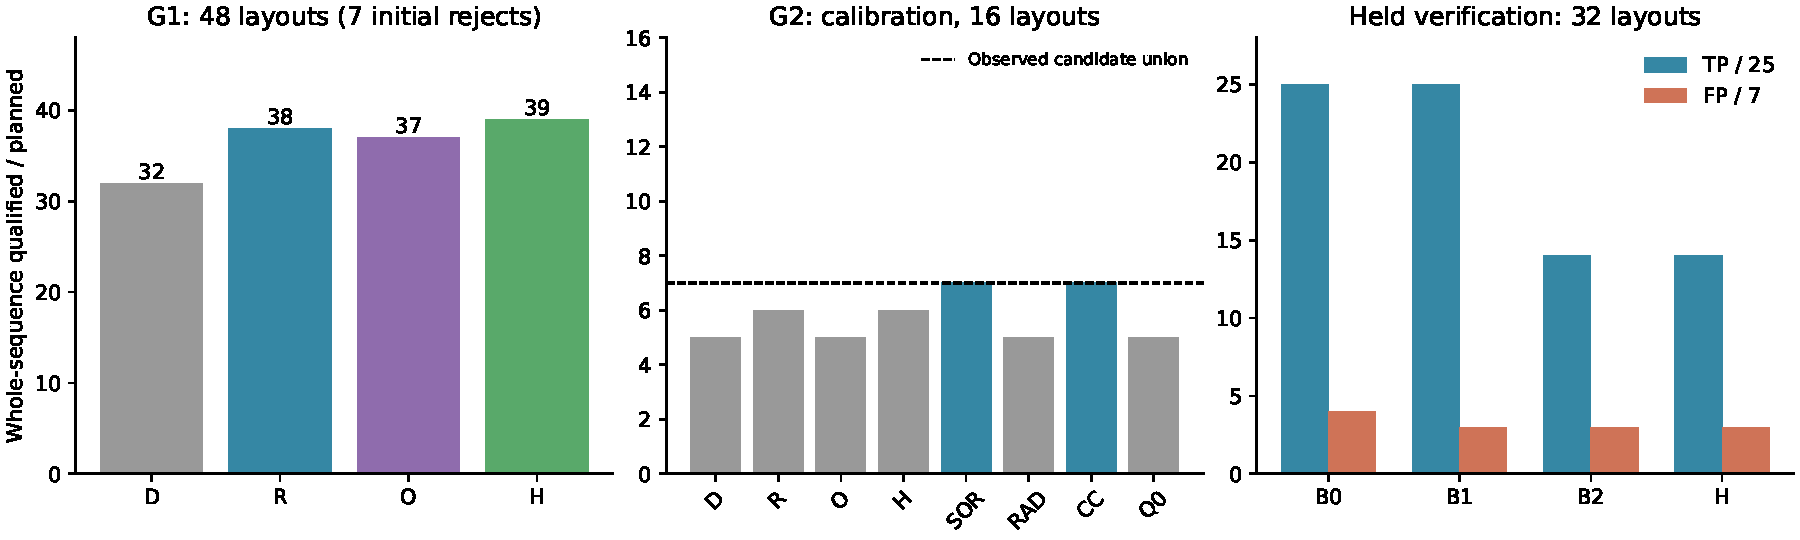
\includegraphics[width=\linewidth]{../figures/diagnostic_results.pdf}\caption{Distinct diagnostic cohorts, not pooled samples. G1 uses 48 planned layouts; G2 is 16 calibration layouts including initial rejects; held verification uses 32 layouts. Counts do not imply statistically significant improvement or full-task success.}\end{figure}
\section*{5. Discussion}

\textbf{Audit the harness before interpreting learning.} Naming an operation \texttt{move} or \texttt{grasp} is insufficient to establish shared semantics across datasets and executors. A schema mismatch is measurable without having a causal estimate of its performance effect. The 450-episode comparison should therefore motivate a matched-executor study, not a claim that parameter deletion would repair the policy.

\textbf{Prefer strong simple controls before a complex selector.} G1's gains over D leave a plausible sensing/processing story, but G2's standard filters match the observed method union. The available evidence does not justify training a more expensive routing model. This is an evidence-based stopping decision, not proof that active perception is generally unnecessary.

\textbf{Measure the full intervention.} Excluding common setup can overstate physical qualification even when every later substep is audited correctly. Scoring-window provenance belongs with the model/configuration provenance. Initialization rejects, unsafe prefixes, process aborts and repeated layouts must remain visible in the accounting.

\textbf{Combine signals only when their error structure supports it.} A fixed AND can reject valid actions when a noisy visual proxy is treated as a necessary condition. A detector that observes an object's visible surface does not automatically track the same physical reference over motion. The current study falsifies this particular conjunction, not multimodal verification as a field.

\section*{6. Limitations and next evidence}

This is a retrospective, single-stack case study. We do not have all three A/R/Q outcomes jointly annotated on one large common cohort, so the three-level model is an organizing contract, not a population estimate of transitions between levels. Multiple studies use different tasks, stages, units and labels; pooling them into one aggregate success rate would be invalid. Development fixes and selected historical cases do not provide population failure frequencies. The task evaluation has one checkpoint/training seed, G1 has two object/task settings, G2 is calibration on four identities, and held detection has only seven negatives. Shared-machine wall time is not pure inference latency.

The numerical release excludes full training trajectories, model checkpoints, CAD/object meshes and raw integration streams pending licensing/dependency closure. Outsiders can reproduce exported tables, not independently reconstruct every physics result from this release alone. The portable utilities illustrate contracts rather than provide a complete turnkey Guava runtime. We report no real-robot validation, learned repair policy, RSI improvement, or completed interface-causality experiment.

A stronger paper would freeze model/prompt/scenes and compare supported extension, explicit rejection, and documented semantic translation, followed by training-seed replication if a training claim is pursued. A generalization claim for filters needs sealed new identities. These are future experiments, not results implied by this draft.

\section*{7. Conclusion}

The Piper migration yields a reusable evidence-audit artifact and several bounded findings: contract divergence is substantial in recorded training data; aggregate task outcomes hide task-specific declines; cheap processing can exhaust the observed benefit of more sensing on a calibration set; and fixed visual--aperture conjunction can lose valid positives without correcting false positives. The useful contribution is an auditable account of these boundaries, not a claimed successful new manipulation method.

\section*{References}

References [1]--[8] are verified against primary sources in \texttt{references.bib} and the reading log. The final venue format, author metadata and reference numbering remain editorial work before submission.

1. Guava: Distilling Frontier VLMs into a Compact Agent through a Robotic Manipulation Harness. \url{https://arxiv.org/abs/2606.18363}
2. robosuite: A Modular Simulation Framework and Benchmark for Robot Learning. \url{https://arxiv.org/abs/2009.12293}
3. LIBERO: Benchmarking Knowledge Transfer for Lifelong Robot Learning. \url{https://arxiv.org/abs/2306.03310}
4. MimicGen: A Data Generation System for Scalable Robot Learning using Human Demonstrations. \url{https://arxiv.org/abs/2310.17596}
5. DROID: A Large-Scale In-The-Wild Robot Manipulation Dataset. \url{https://arxiv.org/abs/2403.12945}
6. Evaluating Real-World Robot Manipulation Policies in Simulation. \url{https://arxiv.org/abs/2405.05941}
7. Deep Reinforcement Learning at the Edge of the Statistical Precipice. \url{https://arxiv.org/abs/2108.13264}
8. Deep Reinforcement Learning that Matters. \url{https://arxiv.org/abs/1709.06560}

\section*{Appendix A. Per-task fixed-checkpoint counts}

\par\noindent\begin{minipage}{\linewidth}\centering\small\setlength{\tabcolsep}{4pt}\begin{tabular}{p{0.370\textwidth}p{0.140\textwidth}p{0.145\textwidth}p{0.145\textwidth}}\hline
Task & Group & Baseline /30 & SFT /30 \\ \hline
apple\_juice\_order & trained & 15 & 17 \\
push\_basket & trained & 1 & 9 \\
red\_objects\_in\_basket & trained & 0 & 0 \\
can\_in\_bin & trained & 1 & 3 \\
close\_drawer & trained & 1 & 2 \\
remove\_cube\_from\_tray & trained & 14 & 2 \\
shell\_game & trained & 0 & 0 \\
pick\_up\_carrot & unseen & 1 & 1 \\
tomato\_near\_potato & unseen & 3 & 6 \\
lemon\_in\_bin & unseen & 0 & 2 \\
push\_pot & unseen & 2 & 14* \\
cube\_stack\_reverse & unseen & 0 & 0 \\
apple\_juice\_reverse\_order & unseen & 11 & 10 \\
bin\_and\_tray\_simple & unseen & 0 & 0 \\
set\_table & unseen & 0 & 0 \\
\hline\end{tabular}\end{minipage}\par\medskip

*Includes one process abort as zero success in the planned denominator, not a fabricated completed official result. Raw per-task counts and source-summary identity hashes are in the release.

\section*{Appendix B. Submission readiness}

The present draft is an empirical technical report. Missing causal ablations, training-seed replication and public raw-physics replay constrain a main-conference claim. An internal CVPR-standard simulated pre-review is provided separately; it is not an official conference review. Human authors must verify manuscript claims, attribution, licensing and AI-assistance disclosure before submission.\end{document}
